\section{Global development paradigms}

Globalization and the implicit challenge of distributed development have become the norm in recent years for large enterprises~\cite{glo24,glo26}.  Evaristo~\cite{glo27} categorizes the nature of these challenges into five critical areas: Perceived distance (geographical and temporal), National culture (languages, accepted work patterns), Development methodology (similarity in processes), Task structure (clarity and structure to team hand-offs) and Organizational distance. The premise is that as the distance between the teams along these critical dimensions increases, the overhead and difficulties associated with distributed development become more prominent. Collaborative development platforms that promote structured interaction between team members can help make distributed development more efficient~\cite{glo28,glo29}. Sharing expertise and the ability to leverage best practices across engagements is a key part of ensuring efficient collaboration -- Expertise Browser~\cite{glo30} and Hipikat~\cite{glo31} are examples of tools that enable sharing at the level of processes and artifacts. Given the rapid churn of resources in the global workforce, a push model of delivering information in situ to developers is important and many of the proposed tools~\cite{glo29,glo31} support this model. The adoption of Cloud, API centric approach to development and agile methods are also helping to reduce the inefficiencies inherent in distributed development. Tooling that can help efficiently leverage a global workforce remains an active and important area of research.

The last few years have seen an accelerated trend towards organizations utilizing a globally integrated development (GID) model for complex IT solution implementation. As with other services, in the first wave of the move towards globally integrated development, the emphasis was on reducing the cost structure through labor arbitrage.  The competition among the major industry players generated the need for aggressive differentiation that goes beyond the benefits of lower cost -- improving quality and reducing time-to-market are becoming key differentiators. In practice, traditional project management techniques that worked well with small co-located teams do not seem to scale well to a global workforce. Practical experience shows that unless development process adopted for GID should be supplemented by an over-arching procedural and architectural framework, that implicitly partitions the development process, it will not be effective. Formal process modeling, strict enforcement of process controls and monitoring the software development process have long been touted as the right way to streamline global delivery~\cite{glo32}. As large enterprises adopted these traditional software delivery models  to distributed development, the natural tendency has been to establish competency centers that cater to specific software skill needs.

As GID matured a second wave of IT services innovation lead to the adoption of software development and deployment practices that improve quality and increase productivity while preserving the advantages of labor arbitrage.  The adoption of a disciplined model for delivery by GID has resulted in new organizational efficiencies, reduced process variance and execution discipline. Figure~\ref{glofig1}, shows the vision of the globally integrated enterprise by focusing on one of the key pain points that inhibit this vision -- a structured way of distributing work to remote teams that promotes collaboration and enforces good governance practices.  Some of the key organizational entities in this approach include: governance and operations teams, a design center that builds the architecture in support of client requirements, and the competency centers which deliver the work. IBM has been a pioneer in this field -- their approach to structured delivery of IT services by a globally distributed delivery team is called application assembly optimization (AAO)~\cite{gloaao}. Other major IT services companies have adopted variations of this same approach.

Work envelopes are central constructs in this approach to structured delivery of software projects that enable disparate competency centers to come together on-demand in the context of a client engagement.  The work envelopes represent a standard envelope by which every work order is authored, transported, and delivered. Work packets include workflow, instruction (normative guidance), metrics collection, and risk management/exception handling mechanisms. Each work envelope constitutes a sub-set of activities that are bound to a larger project plan WBS managed through a traditional project management (PM) tool.

The goals of organizing delivery in this fashion include offering expert guidance through a construct that reduce training time and mentoring, consistent workflow through its governance of process execution and deliverable handoffs, and detailed tracking through timely and accurate windows into task status across globally distributed teams for improved performance and continuous improvement. This approach assumes many of the foundational elements of an organization, and therefore needs governance which integrates into existing governance models at the client IT shop.

\begin{figure}[H]
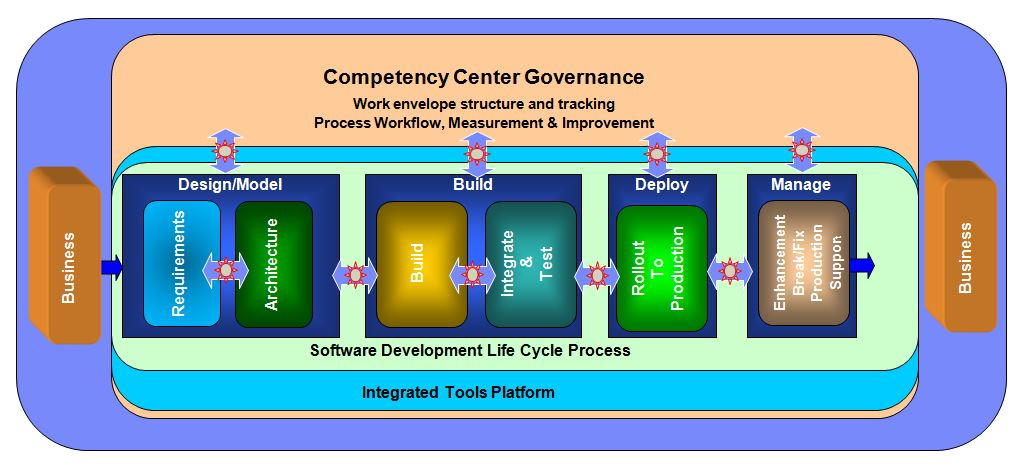
\includegraphics[bb= 0 0 1025 472, scale=0.23]{figs/glocomp.jpg}
\caption{GID model with competency centers}
\label{glofig1}
\end{figure}


\subsection{Research Area: Competency centers}

Although the competency center model has now become central to many IT vendors and large enterprises, it has seen less interest in literature as the focus is on large scale development with a global workforce which is hard to replicate in an academic setting. However, there are several accessible research problems that can significantly improve the performance of these competency centers. We highlight five such problem areas below:

\begin{enumerate}
\item Work envelopes: Central to the concept of a competency center is the ability to partition software projects into granular work envelopes. For certain classes of development and maintenance activities -- for example in the area of packaged applications or SaaS offerings -- partitioning is natural as tasks are repeatable and the skill requirements for a class of tasks is easy to establish. Is there an equivalent construct for more complex software development?
\item Measurement: In large competency centers, performance measurement is key to ensuring efficient operation. In some ways, a competency center, due to the repeatable and comparable nature of tasks it undertakes, makes performance measurement easier. On the other hand, we find that the information reported by the practitioners of a competency center is often unreliable due to the complex structure of incentives involved. Can we take advantage of the structure of a competency center to automate the collection of information to improve its reliability? Can we create checks and balances in the information collected to validate the performance measurement?
\item Estimation: Since competency centers deal with large volumes of tasks belonging to a few categories, it is theoretically possible to create accurate models for estimating the time to complete a development activity. This would vastly improve our ability to predict the effort needed to complete complex software projects.
\item Governance: Enterprises have extended their traditional project management techniques to include competency centers. However, it is unclear whether a project-centric governance model provides the right set of checks and balances to efficiently manage the output of a distributed workforce who are working on several projects at the same time.
\item Planning and scheduling: Traditional calendar day project planning is highly inefficient in the context of a competency center since development tasks can finish either ahead of or behind schedule. Since a practitioner is not tied to a particular project in a competency center, calendar day planning requires constant replanning to ensure that we are fully utilizing available capacity. A better approach would be to use a queue based model, where the queue is managed centrally to re-prioritize the tasks in a practitioner's queue to ensure on time delivery. From a practitioner's perspective, he moves to the next task in the queue once he completes the task at hand -- if he is falling behind, the remaining tasks in his queue can be moved to other practitioners.
\end{enumerate}

\subsection{Towards distributed marketplaces}

The logical evolution of the competency center model that we discussed in the last section is to extend beyond traditional organizational boundaries -- in essence, towards a competitive distributed services marketplace. Instances of such marketplaces are already appearing - for example, services that provide coding expertise for hire such as RentACoder (www.rentacoder.com), TopCoder (www.topcoder.com) are simple examples of this model. Currently, these are seen as a novelty and thus have gained little adoption in large enterprises. In the rest of this section we will explore what it will take to make this mainstream.

 A services delivery marketplace has three key players: provider, consumer and a marketplace enabler. The consumer can use the enabler to ascertain the risks that he is taking in sourcing from a particular provider. The provider in turn gets the ability to competitively price his services based on his delivery record. The enabler provides core enabling services such as: decomposing large or complex projects so they can be executed in parallel by different providers, managing complex projects that are executed in parallel by different providers, providing service level guarantees, or performing service request validation. It is important to note that our marketplace concept is itself an abstraction for efficient service delivery. Thus, all three players can belong to the same organization, each be a different organization in the true global-marketplace sense, or any combination thereof.

 Traditional IT vendors still play a role in this conceptual services marketplace -- however, small or marginal players also have a chance to compete and grow their reputation. In this setup, there are incentives for every one to participate. For traditional IT vendors, it helps offload low margin IT services to smaller vendors with less overhead. For customers it gives an opportunity to out source small work without entering into expensive long term contracts. For the marketplace providers -- who we think will be traditional IT vendors -- it is a chance to profit from helping both providers and consumers take advantage of the marketplace by offering some guarantees.

In contrast to a marketplace for complete products, service delivery is inherently more challenging as it is difficult to capture the intent of the consumer when a service request is created. The service request should not only set forth the details of the work that is to be performed but also make provision to clearly specify risk mitigation, change management, periodic reviews, documentation requirements and exit criteria in a clear fashion to set the right expectations for both the consumer and the provider.  For example, if a code development project being worked on by a provider is not progressing as per the agreed upon schedule agreed upon, a risk mitigation activity may even involve canceling the service agreement. Unless such a risk mitigation activity is clearly spelled out during the creation of the service request, it may open up avenues for misunderstanding. Figure~\ref{glomarketplace} shows the conceptual instantiation of such a marketplace.

 To make this concept practical there are many challenges to be overcome some of which are common to the competency center model. The primary challenge is reducing the overhead required to partition and distribute a large software project into independent units of work that can be done by skilled developers with little or no reference to the overall project context. Open source software development is a case in point where complex software has been developed successfully through a very loosely organized set of developers. For large enterprises, this mode of development may not be suitable as it does not offer appropriate security, governance and schedule controls. Can we find a balance between the need to monitor and manage the outcome with the agility that a truly distributed services marketplace can bring to the table?

 \begin{figure}[H]
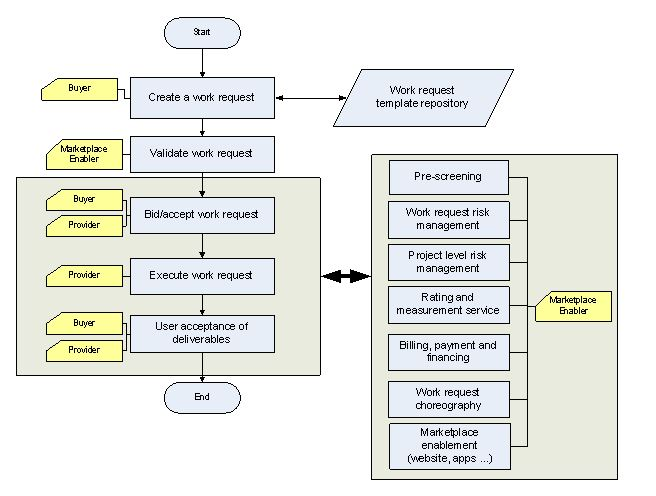
\includegraphics[bb=0 0 656 496, scale=0.4]{figs/glomarketplace.jpg}
\caption{Distributed Services Marketplace}
\label{glomarketplace}
\end{figure}

 Theoretical analysis can point to optimal regimes and controls for the efficient use of a services marketplace. Ranade and Varshney~\cite{glo-ranade} use game theoretic models to offer key insights into some key questions about crowd sourcing in general:what type of tasks should be crowd sourced under what circumstances? Their conclusion is that  the types of tasks (specialized vs generic) and the distribution of skills in the available pool of people will have a big impact on the types of activities that can be effectively outsourced.

\label{sec:global}



